\sys provides compiler support for \emph{automatic task generation} that simplifies writing task-based code by automatically translating C code into a task-based executable. Doing so requires identifying program points to use as task boundaries, defining a set of task functions that begin and end at those boundaries, ensuring that all existing control-flow paths are either contained within a task, or are made explicit in inter-task control-flow, and identifying and instrumenting accesses to task-shared variables that need to be protected by \sys at runtime. The \sys compiler, \textcolor{red}{based on LLVM}, first analyzes the control-flow graph (CFG) and, using a rule-based heuristic, determines at which points to place a task boundary. After identifying where to put task boundaries, the \sys compiler transforms the imperative code into tasks, instrumenting protected memory accesses. 

\subsection{Task Boundary Identification Analysis}
\label{sec:compiler_analysis_pass}

\sys analyzes a program to determine where to put task boundaries to divide the program into tasks. A task is a single-entry, multiple-exit region of the CFG and in a correct task decomposition, no task should ever consume more energy than the device's energy buffer can store. There are several factors that determine whether tasks will execute efficiently. A task decomposition should minimize the number of variables that are accessed by multiple tasks and, consequently, must be protected by \sys's paging mechanism. Tasks should be roughly the same size, simplifying \sys's dynamic reasoning about coalescing by eliminating the need to consider variable task cost at run time. To minimize overhead introduced at task boundaries (i.e., commit), a task decomposition should maximize task size, which minimizes the frequency of task transitions.

%\begin{enumerate}[label={\bf C\arabic*:}]
%\item{No task should ever use up more energy than what the capacitor of the system can provide;} \TODO{We do not (cannot, actually) guarantee this, so I think we can, at best, say that this is an optimization constraint.  What do you think?}
%\item{A task should be single-entry.}\todo{Define single entry}{Kiwan} 
%\end{enumerate}
%
%For a task-decomposition to be efficient, the compiler should optimize the following points:
%
%\begin{enumerate}[label={\bf O\arabic*:}]
%\item{Tasks should be roughly the same size for efficient coalescing;}
%\item{The number of protected variables should be minimized;}
%\item{Task boundary should be visited as least as possible due to overhead on boundaries.}\todo{Define overhead on boundaries}{Kiwan}
%\end{enumerate} 

%\sys meets these correctness and efficiency requirements with a four-part analysis composed of (i) \emph{graph construction}, (ii) \emph{loop analysis}, (iii) \emph{task preparation}, and (iv) \emph{single entry assurance}.

\begin{figure}
	\centering
	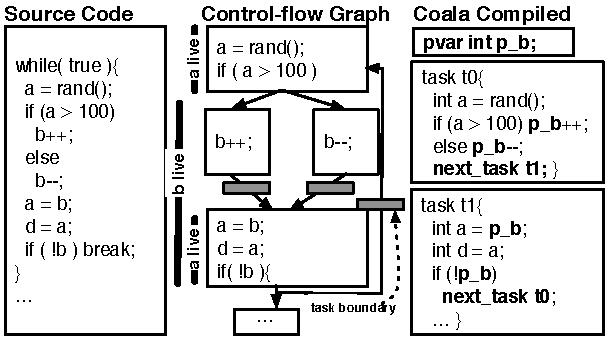
\includegraphics[width=.85\columnwidth]{figures/compiler.pdf}
	\caption{\sys compiles code to use tasks.}
	\label{fig:compiler_overview}
\end{figure}

The input to the task boundary identification analysis is a standard C program (as shown in Figure~\ref{fig:compiler_overview}) and the output of \sys's analysis is the CFG, with some vertices marked as {\em task boundaries}. The \sys compiler builds the program's CFG (as shown in
Figure~\ref{fig:compiler_overview}). To simplify inter-procedural analysis, our prototype inlines all function calls into the main function in the CFG. Recursive function call cannot be handled, so the programmer has to rewrite it into a non-recursive call if there is one. The approach of always inlining function calls will introduce code duplication. If the code size is problematic, alternative approach is to make each function call a task boundary. We leave implementation of such alternative strategy as a future work.
%
%\sys uses a cost-based task boundary placement analysis that considers per-block energy consumption estimates, inter-task variable liveness, and the cost of partitioning loops.
%
We first describe how \sys measures each of these costs and then describe \sys's procedure for placing boundaries in the CFG.

\subsubsection{Task Cost Analysis}

\sys's task cost analysis considers estimated task energy cost, variable liveness, and the impact of splitting loops across tasks. The result of this analysis determines where to place boundaries in the CFG.
 
{\noindent \bf Estimated energy cost.} \sys assigns each basic block in the CFG a {\em cost}, which is an estimate of the energy consumption of the block. Precisely modelling the energy cost of arbitrary C code is a difficult problem and beyond the scope of this work; we simply use the number of intermediate representation (IR) instructions in a block as a proxy for energy because more instructions mean more energy consumption. Moreover, we assume as an input to the compiler the maximum number of operations that the device can execute without exhausting its buffered energy. This parameter is highly device-dependent, and we assume that a developer or device manufacturer determines the number empirically, as we did in this work through direct measurement. \sys's analysis tries to ensure that the estimated energy cost of different tasks is roughly the same and does not exceed given energy budget (which is part of the boundary placement process described later).

{\noindent \bf Live variable cost.} Each CFG edge is associated with a set of variable that {\em may} be {\em alive} across the edge (i.e., variables whose value may be consumed later on). Variables that live across an edge must be protected by \sys's memory virtualization mechanism when boundary is placed at the edge and the resulting inter-task variable increases the run time overhead. \sys's tries to minimize the overhead of protected variables by placing boundaries to minimize the number of inter-task live variables.

{\noindent \bf Loop cost.} Loops are a challenge for \sys because the analysis must account for the cost of multiple iterations of the loop body. \sys assumes that most loops are
annotated with a static loop bound. For loops that do not have a static bound, \sys conservatively assumes the loop will be too large to fit within a single task.

%removed statement "which is common in embedded code"

The analysis tries to minimize the dynamic overhead of traversing task boundaries by avoiding placing a task boundary on a loop with a large bound, when possible. At the same time, the analysis must avoid placing a loop in a single task if the total energy cost of all of its iterations is likely to exceed the device's energy buffer. \sys first multiplies the estimated energy cost of the blocks in the loop body by the loop bound to determine estimate the cost of the loop's execution. If the loop's cost exceeds the device's energy buffer, \sys can place a task boundary on the loop's back-edge, converting each iteration into its own task.  

%of  The reason
%is, if the loop is inside a task it will use up energy that is roughly
%multiplied by the loop count compared to code that is outside of a loop. If the
%resulting cost of a loop is too large\todo{how do you decide on the acceptable
%loop cost?}{Kiwan}, the compiler places boundary at the back edge of the loop,
%and reverts the change to the cost of the vertices inside. It means that if the
%loop is too large to fit in one task, each iteration should be a separate task
%execution.

%If a program has an unbounded loop (such as {\tt while} statement), the compiler conservatively assumes the loop count to be very large. The programmer can prevent this by annotating maximum possible loop count of such unbounded loop if the programmer has the information.\todo{'the' or 'this'? Does it mean programmed still needs to inspect the code?}{Kiwan}

\subsubsection{Task Boundary Placement}
\label{sec:compiler_boundary}

After completing program cost analysis, \sys inserts task boundaries into the CFG in two steps. The first step is to insert task boundaries on the back-edges of all loops that have an energy cost greater than the device's energy buffer capacity, producing an initial boundary placement. The second step is to insert task boundaries at additional points in the code, sub-dividing tasks that have an estimated cost that exceeds the energy buffer's capacity.

To sub-divide these tasks, \sys does depth-first traversals of all paths in the CFG, ignoring back-edges. Traversals start from the beginning of the main function, or from an existing task boundary. \sys accumulates the cost of basic blocks during the traversal until reaching another task boundary or an exit node in the CFG. At the end of a traversal, if the accumulated cost exceeds to device's energy capacity \sys must split the traversed path with a task boundary. Each edge on the path is a candidate location for a boundary.

\sys uses a heuristic to compute a score for each candidate and places a boundary at the candidate with the highest score. The heuristic tries to avoid placing boundaries on loops, to minimize the number of live variables that must be protected across the new boundary, and to maximize the number of operations along the path. A boundary candidate's score is computed as
%
\begin{equation}
\text{score} = {\left(w_{0} N_{\text{IR}} - w_{1} N_{\text{PV}}\right)}{N_{\text{loop}}^{-1}},\nonumber
\end{equation}
%
where $N_{\text{IR}}$ is the length of the path being traversed up to the candidate, $N_{\text{PV}}$ is the number of protected variables that will be newly introduced by placing boundary at the candidate, and $N_{\text{loop}}$ is the product of the loop bounds of all loops (i.e., nested loops) containing the boundary candidate. \sys normalizes $N_{\text{IR}}$ and $N_{\text{PV}}$ to the values among boundary candidates. The weights, $w_{0}, w_{1}$ are between zero and one, and are hand-tuned parameters that define the relative importance of $N_{\text{IR}}$,
$N_{\text{PV}}$, and $N_{\text{loop}}$. We empirically determined these weight values by measuring the runtime for different weight values across applications. We found that varying weights varies runtime by only around 5\% in most cases and in our experimental evaluation, we used $w_{0} = w_{1} = 0.5$.

After placing task boundaries, the compiler must ensure that all tasks are single-entry. To do so, \sys computes the dominator tree of the CFG and checks that every vertex within a task is dominated by the entry vertex of the task. If this dominance condition is unmet for a CFG node, the compiler places an additional task boundary at that node, meeting the condition. Figure~\ref{fig:compiler_overview} illustrates boundary placement: the first three vertices make up one task and the remainder become a second task.

\subsection{Task Transformation}
\label{sec:compiler_transform_pass}

After placing task boundaries during analysis, \sys's transformation analysis restructures the code into tasks defined by the placed boundaries. The analysis traverses the CFG starting from an arbitrary task boundary. On reaching a subsequent boundary, the transformation analysis identifies all paths between the two task boundaries and copies those paths into a new task function. The analysis continues until all paths are contained within a task. 

After forming tasks, variables that are live beyond the end of the task become protected, which requires renaming those variables and updating references to renamed variable names. For example, Figure~\ref{fig:compiler_overview} shows a boundary placed within the live range of {\tt b}; {\tt b} becomes protected and accesses to {\tt b} should be redirected to {\tt p\_b} (as shown in Figure~\ref{fig:compiler_overview}). {\tt a} is task-local and need not be protected, but only declared in the task. Constants and read-only variable are never protected. When writes in multiple, newly formed tasks may update the same location (i.e., at a PHI node in the CFG), \sys re-writes the accesses to refer to the same global name. Subsequent reads simply read the protected variable.

After forming tasks, some branches in a task may refer to targets in another task. \sys patches the CFG to re-write those branches to instead be \transition statements that transition to the entry point of the other task. Such a ``broken'' branch will always refer to a task's entry node because \sys ensures that all tasks have only one entry. 

The compiler re-writes accesses to protected variables to use \sys's memory virtualization API. Pointers pose a challenge to re-writing protected accesses because unprotected pointers may point to protected data. Leveraging LLVM's {\tt basic} pointer alias analysis the compiler conservatively re-writes all accesses that {\em may} read or write protected data. 

%After task generation is done, the compiler generates new main function and
%peppers the system with necessary codes that is needed by \sys (such as code
%for evoking {\tt os\_sceduler}). Also it removes the code that became stale
%(such as the body of a function call, for all the function calls are now
%inlined).

%\subsection{Compiler Design Decisions}
%\label{sec:compiler_limitations}
%
%To be able to implement \sys compiler certain critical assumptions had to be
%made. 
%
%\begin{enumerate}
%	%
%	\item \textbf{Conservative handling of unbounded code sections:} When a C program contains an unbounded loop, the \sys compiler makes a conservative decision of regarding its loop count to be very large. However, if a programmer annotates the expected loop count manually the overhead can be relieved.
%	%
%	\item \textbf{Conservative handling of pointers:} When a C program contains pointer, due to the limitation of pointer alias, the compiler makes the conservative decision. That is, it may consider a variable's live range longer than actual, or it may insert API call for page swap even when it is unnecessary. However, these overhead can be reduced by better pointer aliasing algorithm.
%	%
%	\item \textbf{Function call inlining:} \sys compiler inlines all function call prior to analysis for simplicity. However it can introduce code bloat. Insted, a better way would be to convert large-frequently visited functions to a separate task and make the function call a jump to the task. However we did not implemented such feature for simplicity of the system.
%	%
%	\item \textbf{LLVM IR instruction count to estimate the energy usage:} The compiler uses the number of LLVM IR count as an indicator for energy usage in trying to meet correctness constraint C1 and optimization constraint O1. Intuitively, the number of LLVM IR correlates with the energy usage since more instructions will lead to more energy usage. However, we need to be aware that is nevertheless a crude approach of estimating energy consumption---actual machine instructions are what counts and they are not exactly equal to the LLVM IR. Also, different instructions have different power usage, and even same instruction has different energy usage from time to time (for example cache hit and miss makes even the same {\tt load} instruction to use different amount of energy). However, the energy usage of each task need not be exactly the same to what programmer indicated, and it is sufficient to make sure that all of the tasks are small enough to fit in to the energy budget. Therefore we conjecture that from the \emph{implementation simplicity perspective} of \sys's compiler counting the LLVM IR instruction is sufficient. The programmer can always ensure correctness constraint C1 by conservatively providing IR count in compile time that is empirically proven to be safe. Also, since the estimation of energy usage of each basic block is perpendicular to the compiler itself, it is simple to plug in a better energy model if there is one.
%	%
%	\item \textbf{Limitation of the boundary placement heuristics:} The boundary placement strategy is a heuristic that chooses the local optimum. However, selecting every local optimum might not be the global optimal solution. We can instead do a random search multiple times to find a global optima. Since current heuristic is already showing good result that is comparable to human-written code, refer to Section~\ref{sec:results_coalescing}, we leave such optimization as a future work.
%\end{enumerate}
